\documentclass{beamer}
\usepackage[T1]{fontenc}
\usepackage[english]{babel}
\usepackage{lmodern}
\usepackage{amsmath,amssymb}
\usepackage{algorithm}
\usepackage{algorithmic}
\usepackage{graphicx}
\usepackage{subcaption}
\usepackage{caption}
\usepackage{tikz}
\usetikzlibrary{shapes.geometric,positioning,calc,fit}
\usetikzlibrary{overlay-beamer-styles}
\usepackage{booktabs,multicol,stackengine}
\usepackage[table,dvipsnames]{xcolor}
\usepackage{cancel}
\usepackage{moresize}
\usepackage{hyperref}

\usepackage{listings}
\definecolor{nus-orange}{RGB}{239,124,0}
\definecolor{nus-blue}{RGB}{0,61,124}
\definecolor{halfgray}{gray}{0.55}

\lstset{
  basicstyle=\ttfamily\footnotesize,
  keywordstyle=\bfseries\color{nus-blue},
  stringstyle=\color{ForestGreen},
  numbers=left,
  numberstyle=\scriptsize\color{halfgray},
  rulesepcolor=\color{nus-orange},
  frame=shadowbox,
  columns=flexible,
  showstringspaces=false,
  keepspaces=true,
  tabsize=2,
  breaklines=true
}

\renewcommand{\figurename}{Figure}
\renewcommand{\algorithmname}{Algorithm}

\usepackage{SHU}
\input{macros}

% ---- ER diagram styles (Chen notation, matching the course's official style) ----
\tikzstyle{entity} = [rectangle, draw, thick, minimum width=2.1cm, minimum height=0.8cm, align=center, font=\small]
\tikzstyle{relationship} = [diamond, draw, thick, aspect=2.4, inner sep=1pt, align=center, font=\scriptsize]
\tikzstyle{aggbox} = [draw, thick, inner sep=7pt]
\tikzstyle{eredge} = [-, thick]
\tikzstyle{keydot} = [circle, fill, minimum size=4.5pt, inner sep=0pt]
\tikzstyle{nkdot} = [circle, draw, thick, minimum size=4.5pt, inner sep=0pt]
% #1 unique id, #2 dot style (keydot/nkdot), #3 dot coordinate, #4 label direction (above/below/left/right), #5 label text, #6 entity/box to connect to, #7 overlay step (visible from)
\newcommand{\attrib}[7]{%
  \node[#2, visible on=<#7->] (dot-#1) at #3 {};
  \node[#4=1.5pt of dot-#1, font=\scriptsize, visible on=<#7->] {#5};
  \draw[eredge, visible on=<#7->] (#6) -- (dot-#1);
}
% cardinality label: #1 coordinate, #2 text, #3 overlay step it turns red, #4 = #3+1 (step it turns black)
\newcommand{\cardlabel}[4]{%
  \only<#3>{\node[font=\scriptsize, red] at #1 {#2};}%
  \only<#4->{\node[font=\scriptsize, black] at #1 {#2};}%
}

\title{IT5008: Tutorial 1 --- Entity-Relationship Model}
\author{\href{https://pratik2358.github.io/}{Pratik Karmakar}}
\institute{School of Computing,\\ National University of Singapore}
\date{AY26/27 S1}

\begin{document}

\begin{frame}
  \titlepage
  \IfFileExists{nus-logo.png}{
    \begin{figure}[htpb]\centering
      
\includegraphics[keepaspectratio, scale=0.18]{nus-logo.png}
    \end{figure}
  }{}
\end{frame}

\section{Scenario}

\begin{frame}{The Book Exchange Scenario}
\small
Students at the National University of Ngendipura (NUN) buy books for their studies, and lend/borrow books to/from each other.
\medskip

\textbf{Apasaja Private Limited} is commissioned by the \textbf{NUN Students Association (NUNStA)} to implement an online book exchange system recording:
\begin{itemize}
  \item Information about \textbf{students},
  \item \textbf{Books} that they own,
  \item Books that they \textbf{lend and borrow}.
\end{itemize}
\end{frame}

\begin{frame}{What the Database Must Track}
\small
\begin{itemize}
  \item \textbf{Student}: name, main department, identified by \texttt{email}; \texttt{joined} date; \texttt{graduation} date \emph{if} graduated.
  \item \textbf{Department}: belongs to \emph{exactly one} faculty; no faculty exists without a department; some departments have no students.
  \item \textbf{Book}: title, author(s), publisher, language, year, edition, \texttt{ISBN-10} \emph{and} \texttt{ISBN-13}. Books may exist unowned (owner graduated, or advised but not yet bought).
  \item \textbf{Copy}: a student may own several copies of the \emph{same} book, told apart by a \textbf{copy number} (consecutive from 1).
  \item \textbf{Loan record}: date a copy was borrowed, date it was returned. A student can only borrow/lend \emph{after} being enrolled.
  \item \textbf{Auditing}: keep books/copies/owners as long as owned by a student \emph{or} referenced by a loan; keep graduated students as long as loan records about their books exist.
\end{itemize}
\end{frame}

\section{Constraints}

\begin{frame}{Constraints to Capture}
\small
Before drawing anything, list out the constraints hiding in the text:
\begin{itemize}
  \item Student \texttt{email} uniquely identifies a student.
  \item Book \texttt{ISBN-10} uniquely identifies a book; so does \texttt{ISBN-13}.
  \item A book may be written by \textbf{one or more} authors.
  \item A department belongs to \textbf{exactly one} faculty.
  \item Graduation date is after the joined date. \hfill\emph{(common sense)}
  \item Return date of a loan is after the borrow date. \hfill\emph{(common sense)}
  \item Borrow date is after the joined date.
  \item Copy number is consecutive, starting from 1.
\end{itemize}
\end{frame}

\section{Entity-Relationship Design}

\begin{frame}{Entity Sets}
\small
Nouns (not proper nouns) in the text $\Rightarrow$ entity sets:
\begin{itemize}
  \item \textbf{Students} --- ``\textit{the name and the main department of each student}''; identified by \texttt{email}.
  \item \textbf{Departments} --- ``\textit{A department in NUN must belong to exactly one faculty}''
  \item \textbf{Faculties} --- same quote as above
  \item \textbf{Books} --- ``\textit{the title, author(s), publisher, \dots for each book}''
  \item \textbf{Author} --- ``\textit{author(s)}''
  \item \textbf{Copy} --- ``\textit{We differentiate the copy by its copy number}''
  \item \textbf{Borrow} --- ``\textit{the date at which a book copy is borrowed \dots}''
  \item \textbf{Graduation} / \textbf{Return} --- satellite entities holding the \emph{optional} graduation date and loan-return date (see Design Notes).
\end{itemize}
\end{frame}

\begin{frame}{Relationship Sets}
\small
Verbs / possessive phrases $\Rightarrow$ relationship sets:
\begin{itemize}
  \item \textbf{enroll} --- Students $\leftrightarrow$ Departments: ``\textit{main department of each student}''
  \item \textbf{in} --- Departments $\leftrightarrow$ Faculties: ``\textit{must belong to exactly one faculty}''
  \item \textbf{has} --- Graduation $\leftrightarrow$ Students: ``\textit{If a student has graduated \dots}''
  \item \textbf{own} \emph{(ternary, \alert{aggregate})} --- Students (\emph{owner}), Books, Copy: ``\textit{A student may own multiple copy of the same book}''
  \item \textbf{loan} \emph{(ternary, \alert{aggregate})} --- Students (\emph{borrower}), \textbf{own}, Borrow: ``\textit{We refer to this information as a loan record}''
  \item \textbf{been} --- \textbf{loan} $\leftrightarrow$ Return: ``\textit{the date at which it is returned}''
  \item \textbf{by} --- Books $\leftrightarrow$ Author: ``\textit{author(s)}''
\end{itemize}
\end{frame}

\begin{frame}{Attributes \& Keys}
\small
\begin{tabular}{@{}lll@{}}
\toprule
\textbf{Entity} & \textbf{Attributes} & \textbf{Key} \\
\midrule
Students    & email, join, name       & email \\
Departments & name                    & name \\
Faculties   & name                    & name \\
Graduation  & date                    & date \\
Books       & isbn10, title (\dots), isbn13 & isbn10 \emph{and} isbn13 \\
Author      & name                    & name \\
Copy        & copy num                & copy num \\
Borrow      & date                    & date \\
Return      & date                    & date \\
\bottomrule
\end{tabular}
\vspace{0.5em}

{\scriptsize $\bullet$ = key attribute \quad $\circ$ = non-key attribute (matches the diagram notation)}
\end{frame}

\begin{frame}{ER Notation Legend}
\begin{center}
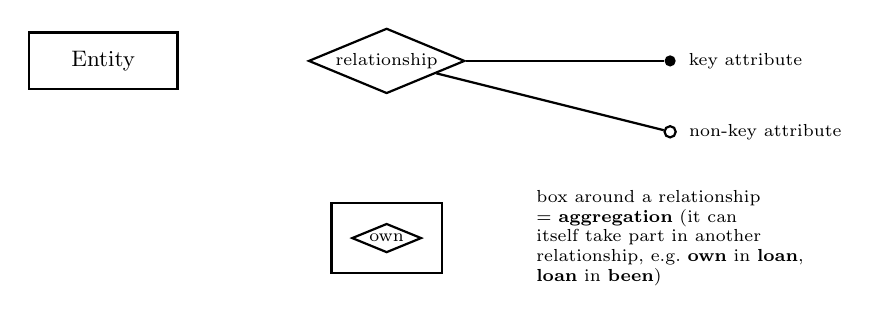
\begin{tikzpicture}[scale=0.9, every node/.style={transform shape}]
  \node[entity] (e1) at (0,0) {Entity};
  \node[relationship] (r1) at (4,0) {relationship};
  \attrib{leg-key}{keydot}{(8,0)}{right}{key attribute}{r1}{1}
  \attrib{leg-nk}{nkdot}{(8,-1)}{right}{non-key attribute}{r1}{1}
  \node[relationship] (r2) at (4,-2.5) {own};
  \node[aggbox, fit=(r2)] {};
  \node at (8,-2.5) [font=\scriptsize, align=left] {box around a relationship\\= \textbf{aggregation} (it can\\itself take part in another\\relationship, e.g.\ \textbf{own} in \textbf{loan},\\\textbf{loan} in \textbf{been})};
\end{tikzpicture}
\end{center}
\vspace{0.3em}
\small
Rectangle = entity set. Diamond = relationship set. $\bullet$ = key attribute, $\circ$ = non-key attribute (text sits beside the dot, connected straight to the entity/relationship). Edge labels give (min,max) participation. \textbf{own} and \textbf{loan} are \emph{ternary} (three participants each).
\end{frame}

\begin{frame}{Entity-Relationship Diagram}
\begin{center}
\resizebox{\linewidth}{!}{%
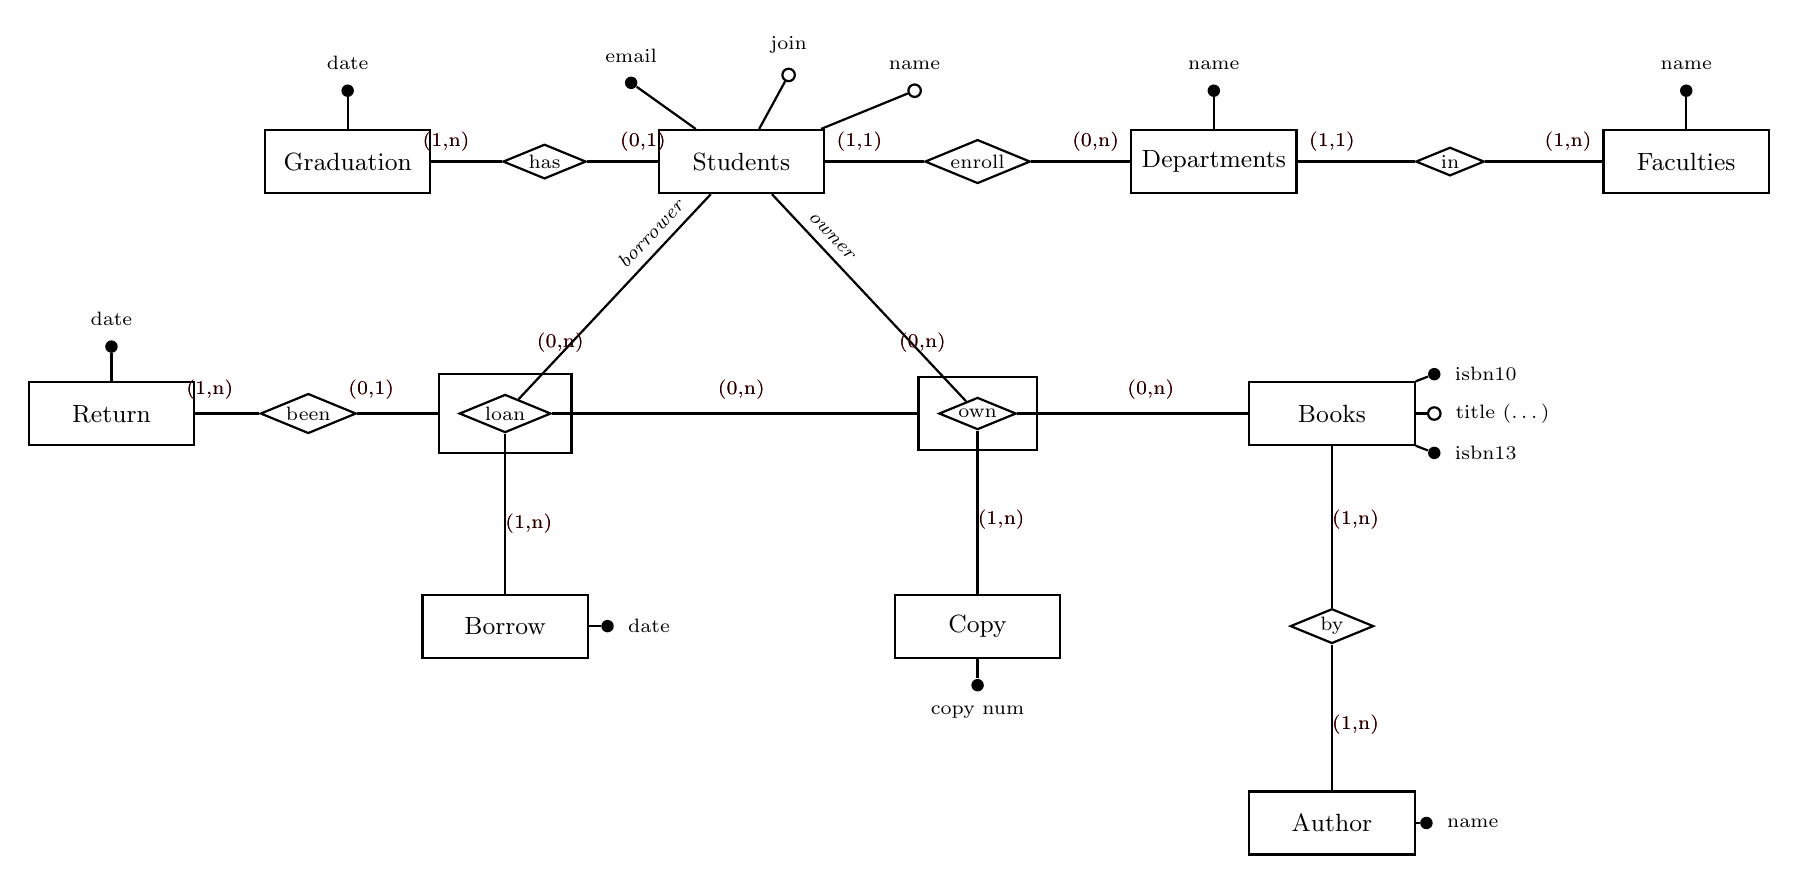
\begin{tikzpicture}
  % ==== PHASE 1: structure, one item at a time (steps 1-16) ====
  % 1.Students 2.Departments 3.enroll 4.Faculties 5.in 6.Graduation 7.has
  % 8.Books 9.Author 10.by 11.Copy 12.own 13.Borrow 14.loan 15.Return 16.been
  \node[entity, visible on=<1->] (student) at (0,9) {Students};
  \node[entity, visible on=<2->] (department) at (6,9) {Departments};
  \node[relationship, visible on=<3->] (enroll) at (3,9) {enroll};
  \draw[eredge, visible on=<3->] (student) -- (enroll);
  \draw[eredge, visible on=<3->] (enroll) -- (department);
  \node[entity, visible on=<4->] (faculty) at (12,9) {Faculties};
  \node[relationship, visible on=<5->] (in) at (9,9) {in};
  \draw[eredge, visible on=<5->] (department) -- (in);
  \draw[eredge, visible on=<5->] (in) -- (faculty);
  \node[entity, visible on=<6->] (graduation) at (-5,9) {Graduation};
  \node[relationship, visible on=<7->] (has) at (-2.5,9) {has};
  \draw[eredge, visible on=<7->] (graduation) -- (has);
  \draw[eredge, visible on=<7->] (has) -- (student);
  \node[entity, visible on=<8->] (books) at (7.5,5.8) {Books};
  \node[entity, visible on=<9->] (author) at (7.5,0.6) {Author};
  \node[relationship, visible on=<10->] (by) at (7.5,3.1) {by};
  \draw[eredge, visible on=<10->] (books) -- (by);
  \draw[eredge, visible on=<10->] (by) -- (author);
  \node[entity, visible on=<11->] (copy) at (3,3.1) {Copy};
  \node[relationship, visible on=<12->] (own) at (3,5.8) {own};
  \node[aggbox, fit=(own), visible on=<12->] (ownbox) {};
  \draw[eredge, visible on=<12->] (student) -- node[above,sloped,pos=0.25]{\scriptsize\itshape owner} (own);
  \draw[eredge, visible on=<12->] (own) -- (books);
  \draw[eredge, visible on=<12->] (own) -- (copy);
  \node[entity, visible on=<13->] (borrow) at (-3,3.1) {Borrow};
  \node[relationship, visible on=<14->] (loan) at (-3,5.8) {loan};
  \node[aggbox, fit=(loan), visible on=<14->] (loanbox) {};
  \draw[eredge, visible on=<14->] (student) -- node[above,sloped,pos=0.25]{\scriptsize\itshape borrower} (loan);
  \draw[eredge, visible on=<14->] (loan) -- (ownbox.west);
  \draw[eredge, visible on=<14->] (loan) -- (borrow);
  \node[entity, visible on=<15->] (return) at (-8,5.8) {Return};
  \node[relationship, visible on=<16->] (been) at (-5.5,5.8) {been};
  \draw[eredge, visible on=<16->] (return) -- (been);
  \draw[eredge, visible on=<16->] (been) -- (loanbox.west);

  % ---- attributes, tied to their entity's own step ----
  \attrib{s-email}{keydot}{(-1.4,10.0)}{above}{email}{student}{1}
  \attrib{s-join}{nkdot}{(0.6,10.1)}{above}{join}{student}{1}
  \attrib{s-name}{nkdot}{(2.2,9.9)}{above}{name}{student}{1}
  \attrib{d-name}{keydot}{(6,9.9)}{above}{name}{department}{2}
  \attrib{f-name}{keydot}{(12,9.9)}{above}{name}{faculty}{4}
  \attrib{g-date}{keydot}{(-5,9.9)}{above}{date}{graduation}{6}
  \attrib{b-isbn10}{keydot}{(8.8,6.3)}{right}{isbn10}{books}{8}
  \attrib{b-title}{nkdot}{(8.8,5.8)}{right}{title (\dots)}{books}{8}
  \attrib{b-isbn13}{keydot}{(8.8,5.3)}{right}{isbn13}{books}{8}
  \attrib{a-name}{keydot}{(8.7,0.6)}{right}{name}{author}{9}
  \attrib{c-num}{keydot}{(3,2.35)}{below}{copy num}{copy}{11}
  \attrib{bo-date}{keydot}{(-1.7,3.1)}{right}{date}{borrow}{13}
  \attrib{r-date}{keydot}{(-8,6.65)}{above}{date}{return}{15}

  % ==== PHASE 2: participation constraints, one at a time, red then black (steps 17-32) ====
  \cardlabel{(1.5,9.25)}{(1,1)}{17}{18}    % 1. Students -- enroll
  \cardlabel{(4.5,9.25)}{(0,n)}{18}{19}    % 2. Departments -- enroll
  \cardlabel{(-1.25,9.25)}{(0,1)}{19}{20}  % 3. Students -- has
  \cardlabel{(-3.75,9.25)}{(1,n)}{20}{21}  % 4. Graduation -- has
  \cardlabel{(7.5,9.25)}{(1,1)}{21}{22}    % 5. Departments -- in
  \cardlabel{(10.5,9.25)}{(1,n)}{22}{23}   % 6. Faculties -- in
  \cardlabel{(-2.3,6.7)}{(0,n)}{23}{24}    % 7. loan -- Students (borrower)
  \cardlabel{(2.3,6.7)}{(0,n)}{24}{25}     % 8. own -- Students (owner)
  \cardlabel{(5.2,6.1)}{(0,n)}{25}{26}     % 9. Books -- own
  \cardlabel{(7.8,4.45)}{(1,n)}{26}{27}    % 10. Books -- by
  \cardlabel{(7.8,1.85)}{(1,n)}{27}{28}    % 11. Author -- by
  \cardlabel{(3.3,4.45)}{(1,n)}{28}{29}    % 12. own -- Copy
  \cardlabel{(0,6.1)}{(0,n)}{29}{30}       % 13. loan -- own
  \cardlabel{(-2.7,4.4)}{(1,n)}{30}{31}    % 14. loan -- Borrow
  \cardlabel{(-4.7,6.1)}{(0,1)}{31}{32}    % 15. loan -- been
  \cardlabel{(-6.75,6.1)}{(1,n)}{32}{33}   % 16. Return -- been
\end{tikzpicture}}
\end{center}
\vspace{0.3em}
{\footnotesize\color{red}\centering
\only<17>{Every student enrolls in exactly one department.}%
\only<18>{A department may have zero students.}%
\only<19>{A student may or may not have graduated yet.}%
\only<20>{We only store a graduation date once it exists.}%
\only<21>{A department belongs to exactly one faculty.}%
\only<22>{No faculty exists without at least one department.}%
\only<23>{A student may hold zero or many loans.}%
\only<24>{A student may own zero or many copies.}%
\only<25>{A book may exist with zero owned copies.}%
\only<26>{A book is written by one or more authors.}%
\only<27>{An author is only recorded once they've written a book.}%
\only<28>{own has no meaning without a copy --- forces a merge later.}%
\only<29>{A copy may be loaned zero or many times.}%
\only<30>{loan has no meaning without a borrow date --- forces a merge later.}%
\only<31>{A loan may not yet have been returned.}%
\only<32>{We only store a return date once it is actually returned.}%
\par}
\end{frame}

\begin{frame}{Design Notes --- Ternary Relationships \& Aggregation}
\small
\begin{itemize}
  \item \textbf{own} and \textbf{loan} are \emph{ternary}: a student owning/borrowing involves \emph{three} participants at once (student, book/copy, and the copy/borrow event) --- a binary relationship cannot express that.
  \item \textbf{Two} relationships must be boxed as \textbf{aggregates}, because each is itself a participant in a further relationship (a plain relationship cannot connect directly to another relationship):
  \begin{itemize}
    \item \textbf{own} $\to$ boxed, because \textbf{loan} needs to reference ``this particular owned copy'' as a whole, not just \texttt{Students} or \texttt{Copy} alone.
    \item \textbf{loan} $\to$ also boxed, because \textbf{been} needs to reference ``this particular loan event'' as a whole, not just \texttt{Students}, \texttt{own}, or \texttt{Borrow} alone.
  \end{itemize}
  \item \textbf{Students} plays two \emph{roles}: \emph{owner} (into \textbf{own}) and \emph{borrower} (into \textbf{loan}) --- same entity set, two different participations.
\end{itemize}
\end{frame}

\begin{frame}{Design Notes --- Optional Attributes as Satellite Entities}
\small
\begin{itemize}
  \item \textbf{Graduation} $\to$ \textbf{has} $\to$ \textbf{Students} is \textbf{(1,n)}--\textbf{(0,1)}: a student may or may not have graduated, and we don't want to store an unused graduation date on every student row. Same reasoning for \textbf{Return} $\to$ \textbf{been} $\to$ \textbf{loan}.
  \item These \textbf{(1,n)} satellite entities (Graduation, Return, and likewise Copy into \textbf{own}, Borrow into \textbf{loan}) are designed to be \emph{merged} into their relationship at the logical-design stage --- see next section.
\end{itemize}
\end{frame}

\section{Logical Design}

\begin{frame}[fragile]{Relational Schema --- Department, Student}
\begin{lstlisting}[language=SQL]
CREATE TABLE department (
  faculty VARCHAR(62) NOT NULL,
  name    VARCHAR(32) PRIMARY KEY
);

CREATE TABLE student (
  name       VARCHAR(32) NOT NULL,
  email      VARCHAR(256) PRIMARY KEY,
  year       DATE NOT NULL,       -- join date
  graduate   DATE CHECK (graduate >= year),
  department VARCHAR(32) NOT NULL
    REFERENCES department(name)
);
\end{lstlisting}
\textbf{Deviation:} \texttt{department}--\texttt{faculty} and \texttt{student}--\texttt{Graduation} are each merged into one table (the (1,1) side has no attributes of its own to justify a separate table; merging \texttt{graduate} lets us write the \texttt{CHECK} in one place).
\end{frame}

\begin{frame}[fragile]{Relational Schema --- Book, Author}
\begin{lstlisting}[language=SQL]
CREATE TABLE book (
  title     VARCHAR(256) NOT NULL,
  publisher VARCHAR(64)  NOT NULL,
  language  VARCHAR(32)  NOT NULL,
  year      DATE NOT NULL,
  edition   INT  NOT NULL,
  isbn10    CHAR(10) NOT NULL UNIQUE,
  isbn13    CHAR(14) PRIMARY KEY
);

CREATE TABLE author (
  name VARCHAR(32),
  book CHAR(14) REFERENCES book(isbn13),
  PRIMARY KEY (name, book)
);
\end{lstlisting}
\end{frame}

\begin{frame}[fragile]{Relational Schema --- own\_copy, loan}
\begin{lstlisting}[language=SQL]
CREATE TABLE own_copy (
  owner VARCHAR(256) REFERENCES student(email),
  book  CHAR(14) REFERENCES book(isbn13),
  copy  INT CHECK (copy > 0),
  PRIMARY KEY (owner, book, copy)
);

CREATE TABLE loan (
  borrower VARCHAR(256) REFERENCES student(email),
  owner    VARCHAR(256),
  book     CHAR(14),
  copy     INT,
  borrowed DATE,
  returned DATE CHECK (returned >= borrowed),
  FOREIGN KEY (owner, book, copy)
    REFERENCES own_copy(owner, book, copy),
  PRIMARY KEY (borrowed, borrower, owner, book, copy)
);
\end{lstlisting}
\textbf{Deviation:} \textbf{own} (ternary, aggregate) becomes \texttt{own\_copy} --- it \emph{is} the Copy entity, since a copy never exists without an owner. \textbf{loan} absorbs \textbf{Borrow} and \textbf{Return} the same way.
\end{frame}

\begin{frame}{Constraints Not Captured by the DDL}
\small
\begin{itemize}
  \item \textbf{Copy number is consecutive from 1} --- needs the values across \emph{all} rows for an (owner, book); a single-row \texttt{CHECK} cannot see other rows.
  \item \textbf{Borrow date is after the joined date} --- compares columns across \texttt{loan} and \texttt{student}; a single-row \texttt{CHECK} cannot reach into another table.
  \item \texttt{graduate >= year} and \texttt{returned >= borrowed} \textbf{are} captured, via same-row \texttt{CHECK} constraints.
  \item \textbf{Audit retention} (keep books/copies/students while referenced by a copy or loan) is captured \emph{implicitly}: the default foreign-key behaviour (\texttt{ON DELETE RESTRICT}) blocks any \texttt{DELETE} that would orphan an \texttt{own\_copy} or \texttt{loan} row.
\end{itemize}
\end{frame}

\begin{frame}
\begin{center}
Questions?\\
Drop a mail at: pratik.karmakar@u.nus.edu
\end{center}
\end{frame}

\end{document}
